\documentclass[a4paper,10pt]{article}
\usepackage[paperwidth=210mm, paperheight=297mm, left=2.5cm, top=2.5cm, right=2.5cm, bottom=1.0cm, head=1.5cm, includefoot]{geometry}
%\usepackage[latin1]{inputenc}

\usepackage[english]{babel}
\usepackage[utf8x]{inputenc}
\usepackage{amsmath}

\usepackage{mathtools}
\DeclarePairedDelimiter\ceil{\lceil}{\rceil}
\DeclarePairedDelimiter\floor{\lfloor}{\rfloor}

\usepackage{bookman}
\usepackage{booktabs}
\usepackage[pdfborder={0 0 0}]{hyperref}
\usepackage{pdfpages}
\usepackage{fancyhdr}
\usepackage{lastpage}
\usepackage{verbatim}
\usepackage{graphicx}
\usepackage{fixltx2e}
\usepackage{listings}

%\usepackage[T1]{fontenc}
%\usepackage{comment}
%\usepackage{makeidx}
%\usepackage{float}
%\usepackage{slashbox}

\renewcommand{\headrulewidth}{1pt}
\renewcommand{\footrulewidth}{1pt}



%%%%%%%%%  Datos  %%%%%%%%%

\title{ \textbf{Trabajo práctico 1: Conjunto de instrucciones MIPS} }

\author{Contini, Agustín - \textit{Padrón 89180}			\\
            \texttt{ agscontini@gmail.com }				\\
            Farina, Federico - \textit{Padrón 90177}			\\
            \texttt{ federicojosefarina@gmail.com }				\\
            Prystupiuk, Maximiliano  - \textit{Padrón 94853  }			\\
            \texttt{ mprystupiuk@gmail.com  }					\\[2.5ex]
            1er. Cuatrimestre de 2017					\\[1.0ex]
            \normalsize{66.20 Organización de Computadoras}		\\
            \normalsize{Facultad de Ingeniería, Universidad de Buenos Aires}	\\
	}
\date{\today}

%%%%%%%%%  Fin datos  %%%%%%%%%



\begin{document}



%%%%%%%%%  1era hoja: caratula y datos  %%%%%%%%%

\maketitle
\bigskip
\thispagestyle{empty}	% quita el numero en la primera pagina

\begin{abstract}
El trabajo consiste conseguir que un conjunto de programas
cumplan con una condición, cuando normalmente no lo harían, aprovechando las vulnerabilidades del stack y de la función gets() teniendo un buffer de largo fijo y conocido.
Para este cometido se utilizará gdb y objdump como herramientas sobre MIPS32 en un entorno NetBSD.

\end{abstract}



%%%%%%%%%  Fin 1era hoja  %%%%%%%%%



%%%%%%%%%  Head y foot  %%%%%%%%%

\pagestyle{fancy}
\lhead{
\includegraphics[width=1.2cm]{./img/logo.png}}
\chead{Trabajo práctico 1: Conjunto de instrucciones MIPS \\ \textit{Contini  -  Farina  -  Prystupiuk} }

\rfoot{$1^{er}$ Cuatrimestre 2017}
\lfoot{66.20 Organizaci\'on de Computadoras}
\cfoot{\hspace{2.4cm}   P\'agina \thepage \, de \pageref{LastPage} }

%%%%%%%%%  Fin head y foot  %%%%%%%%%



\normalsize

\newpage
\tableofcontents	% hoja de indices de titulos, subtitulos

\vspace{2.0cm}
\listoffigures		% hoja de indices de figuras

\newpage
\section{Introducci\'on}

\subsection{Problemas de programación insegura}

Los ejercicios a analizar fueron diseñados especialmente para la compresión del funcionamiento de los programas compilados en C por Gerardo Richarte y son de especial interés para la compresión del stack y la explotación de sus vulnerabilidades.
\par El trabajo consiste en conseguir que los programas stack1.c a stack5.c cumplan una condición y impriman la frase "you win!" aprovechando que utilizan la función gets para llenar un buffer de largo fijo y conocido utilizando gdb para examinar el stack y los valores de los registros y objdump para inspeccionar de manera sencilla las posiciones relativas al stack pointer.


\newpage
\section{Uso}
\subsection{Compilado}
Ofrecemos dos formas de correr el trabajo práctico:
\begin{enumerate}
\item  Correr el run.sh dentro del entorno de NetBSD, en el directorio del proyecto, ejecutando:
	\begin{verbatim}
$ ./run.sh
\end{verbatim}
\item Dentro del entorno de NetBSD, en el directorio del proyecto ejecutar para cada archivo i:
\begin{verbatim}
$ gcc -g stack{i}.c -o stack{i}.o
\end{verbatim}
\end{enumerate}



\subsection{Herramientas utilizadas}
\subsubsection{GDB}

GDB (Gnu Project Debugger) es una herramienta que permite entre otras cosas, correr el programa con la posibilidad de detenerlo cuando se cumple cierta condición, avanzar paso a paso y, entre otras cosas, analizar el stack frame actual de cada uno de ellos. También te permite, en caso de fallar el programa y habiendo sido levantado con la herramienta, conocer el estado de lo que ocurrió y produjo el fallo.


\subsubsection{Objdump}

Objdump es una herramienta muy útil que despliega información sobre uno o más archivos objeto de manera que nos permite ver el código assembler en ellos. Posee otras funcionalidades para ver información sobre archivos con código, pero nuestro uso se limito a ver el código assembler de los archivos, ya que nos daba la información necesaria para trabajar.

\newpage
\section{Programas}
\subsection{stack1}
\lstset{ language = C, numbers=left, tabsize=4, breaklines=true, frame=single }
\lstinputlisting{./stack1.c}

\subsubsection{Descripción}

\bigskip
Mediante gdb podemos ver que la disposición del stack frame para este programa es la siguiente

\bigskip

\begin{figure}[h!]
	\centering
	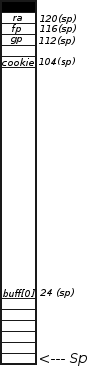
\includegraphics[scale=0.7]{./recursos/stack1.png}
	\caption{Gr\'afico del stack del programa stack1}
    \label{fig:stack1}
\end{figure}


\bigskip
Lo que nos dice que las posiciones del array del buffer siguen la disposición:

\begin{equation*}
\forall x \in [0,n], \quad \&buff[x]=sp(24+ 4 * \floor*{\frac{x}{4}})
\end{equation*}


\subsubsection{Solución}

Al crecer las posiciones del array hacia arriba en el stack lo único que debemos hacer es escribir el buffer en la posición x=80  para que la última word coincida con la posición de memoria de cookie, en la posición 104(sp), y luego hacer que corresponda con el hexadecimal 0x41424344 que es el codigo ascci correspondiente al texto ABCD.
\bigskip
Una manera de comprobar esto es ejecutar las siguientes lineas en una consola:

\begin{lstlisting}
input = "0000000000000000000000000000000000000000
0000000000000000000000000000000000000000DCBA"
echo $input | ./stack1.o
\end{lstlisting}

O escapeando y en hexadecimal:

\begin{lstlisting}
input = "0000000000000000000000000000000000000000
0000000000000000000000000000000000000000\x44\x43\x42\x41"
echo -e $input | ./stack1.o
\end{lstlisting}

\bigskip

Lo que en ambos casos resultará en el output: "you win!"


\subsection{stack2}
\lstset{ language = C, numbers=left, tabsize=4, breaklines=true, frame=single }
\lstinputlisting{./stack2.c}

\subsubsection{Descripción}

El stack será el mismo que el de la figura \textbf{(\ref{fig:stack1})}. La diferencia en este programa es que no inicializamos con un valor a cookie, pero al tener que sobreescribirlo nos es indistinto.

\subsubsection{Solución}

En este caso el hexadecimal que queremos que esté en la posición sp(104) es el 0x01020305, por lo tanto una posible solución es:

\begin{lstlisting}
input = "0000000000000000000000000000000000000000
0000000000000000000000000000000000000000\x05\x03\x02\x01"
echo -e $input | ./stack2.o
\end{lstlisting}
\bigskip

Lo que resultará en el output: "you win!"

\subsection{stack3}
\lstset{ language = C, numbers=left, tabsize=4, breaklines=true, frame=single }
\lstinputlisting{./stack3.c}

\subsubsection{Descripción}
Al igual que en los casos anteriores, el stack será el mismo que el de la figura \textbf{(\ref{fig:stack1})}.
\subsubsection{Solución}

El hexadecimal a escribir en esta caso es 0x01020005, de manera que una posible solución será: 

\begin{lstlisting}
input = "0000000000000000000000000000000000000000
0000000000000000000000000000000000000000\x05\x00\x02\x01"
echo -e $input | ./stack3.o
\end{lstlisting}

\bigskip

Lo que resultará en el output: "you win!"

\subsection{stack4}
\lstset{ language = C, numbers=left, tabsize=4, breaklines=true, frame=single }
\lstinputlisting{./stack4.c}


\subsubsection{Descripción}

\begin{figure}[h!]
	\centering
	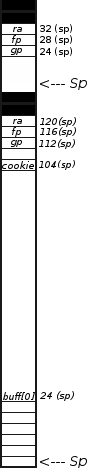
\includegraphics[height=9cm]{./recursos/stack4.png}
	\caption{Gr\'afico del stack del programa stack4}
    \label{fig:stack4}
\end{figure}

Este es el primer caso en el que tenemos dos stack frames, uno del \textbf{main} y otro que le corresponde a \textbf{stack4()}. 

\subsubsection{Solución}

Este caso es diferente a los anteriores porque el hexadecimal que espera cookie contiene el caracter 0x0A, que corresponde a un \textbf{line feed}, y por lo tanto no es un input válido para el \textbf{gets}.
La solución en este caso es escribir directamente el \textbf{ra} con la posición de memoria donde se encuentra el "you win". 

Se puede ver tambien en el stack que ra se encuentra a 96 posiciones del inicio de buff0. Sabiendo esto y usando el \textbf{objdump} para obtener la posición de memoria correspondiente a la frase, una posible solución es:

\begin{lstlisting}
perl -e 'print "a"x96 . "\x40\x0c\x40\x00"' | ./a.out
\end{lstlisting}

\bigskip

Lo que resultará en el output: "you win!"

\subsection{stack5}

\lstset{ language = C, numbers=left, tabsize=4, breaklines=true, frame=single }
\lstinputlisting{./stack5.c}

\lstset{ language = C, numbers=left, tabsize=4, breaklines=true, frame=single }
\lstinputlisting{./stack5.h}

\lstset{ language = C, numbers=left, tabsize=4, breaklines=true, frame=single }
\lstinputlisting{./win.h}

\lstset{ language = C, numbers=left, tabsize=4, breaklines=true, frame=single }
\lstinputlisting{./win.c}

\newpage
\section{Conclusión}

   Como se puede apreciar, y como bien se aclara en el enunciado, y advierte NetBSD al compilar los programas, utilizar gets() es inseguro y no recomendable (hoy en día arreglado en los sistemas operativos) ya que abre la vulnerabilidad de ingresar información externa directamente en el stack del programa, logrando incluso poner código ejecutable en el mismo, pudiendo lograr el control del flujo del programa. 
   \newline
  Esta vulnerabilidad, y el uso de las herramientas gdb y objdump nos permitieron ver la manera de en los cinco casos conocer el stack, ver donde estaba la información que necesitabamos y que era lo que debíamos inyectar para obtener el resultado que buscabamos.  
    En los primero tres casos, con identificar cual era la cookie que debía coincidir y completando esos pocos valores sobrepasando el buffer con la funcion gets(), nos bastó con un echo con pipe a la ejecución del programa.
    \newline
   En los últimos dos casos nos valimos de perl para inyectar la información en el buffer, porque resulta menos tedioso para completar la información necesaria, además de ser un caso más general (si el buffer fuera $n$ bytes el ingreso a mano no es rentable) \newline
   Cabe destacar que el uso de echo es necesario para los casos 2 en adelante, ya que deben ingresarse carácteres que normalmente no podrían mandarse por el teclado.\newline
   En el caso stack2, podría haberse realizado la entrada mediante $[...]000^{\circ}E^{\circ}C^{\circ}B^{\circ}A$
   , siendo:
   
   $^{\circ}E: ctrl+shift+E$
    
   $^{\circ}C: ctrl+shift+C$
   
   $^{\circ}B: ctrl+shift+B$
   
   $^{\circ}A: ctrl+shift+A$
   
   Pero el problema surge en $ctrl+shift+C$, ya que $ctrl+C$ produce la $SignalTrap$ 2, INT (que interrumpe la ejecución del programa). \newline
   Es por eso que se envían los caracteres desde echo con las opciones $-ne$ para interpretar las secuencias de escape y poder mandar los caracteres con su codificacion en HEX mediante \\xFF.
  \newline Stack 4 agrega la dificultad de necesitar mandar "0a", que es el LineFeed, y se almacena como 00 por estar mandando texto en una consola. Es por esto que en vez de modificar el valor de la cookie se modificó la dirección dónde se almacena ra (return andress) con la posición de memoria de la función que imprime el mensaje ganador.
   \newline Stack 5 es similar, pero al ser sólo una función necesita un main que la llame. Respetando la consigna, se compiló stack5.c como se encuentra, pero la función main.c que la llama incluye a su vez una función win() que imprime lo deseado. Por lo que de manera análoga al caso 4, pasando la dirección de memoria de la función en el valor dónde se almacena ra en el stack puedo romper el flujo de ejecución del programa con mucha libertad.
   








\end{document}
